% 2015_shaanxi_science_q18: Fig1 right trapezoid + diagonals; Fig2 folded tetrahedron-like solid
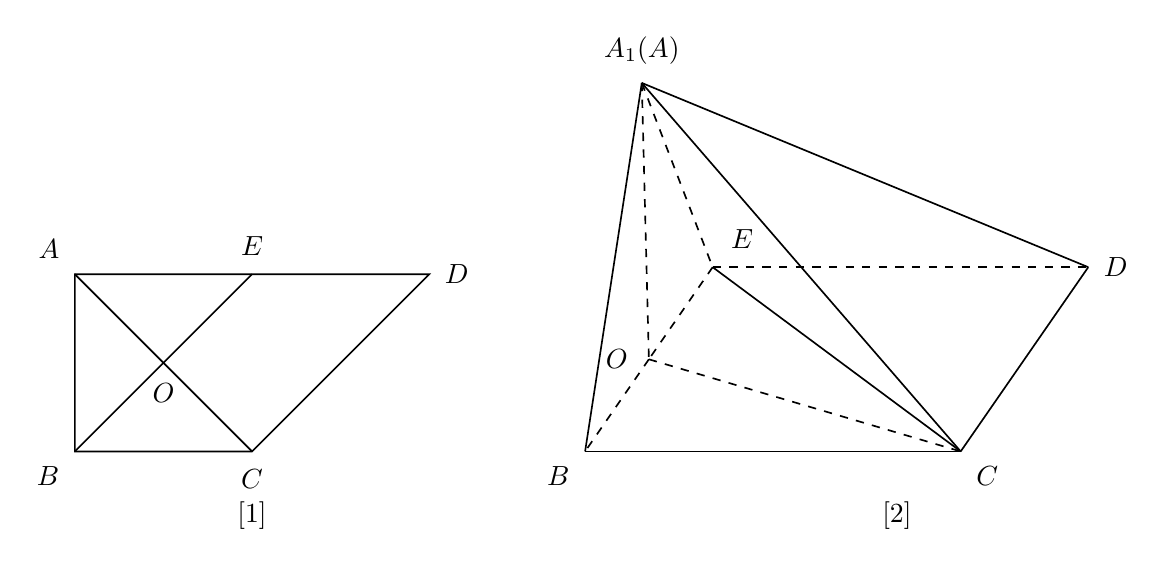
\begin{tikzpicture}[x=.9cm,y=.9cm,line width=0.6pt, font=\normalsize]
% ---- panel 1: plane figure ----
\coordinate (P1A) at (0,2.5);
\coordinate (P1E) at (2.5,2.5);
\coordinate (P1D) at (5,2.5);
\coordinate (P1B) at (0,0);
\coordinate (P1C) at (2.5,0);
\coordinate (P1O) at (1.25,1.25);
\draw (P1A)--(P1E)--(P1D)--(P1C)--(P1B)--cycle;
\draw (P1A)--(P1C);
\draw (P1B)--(P1E);
\node[above left=2pt] at (P1A) {$A$};
\node[below left=2pt] at (P1B) {$B$};
\node[below=3pt] at (P1C) {$C$};
\node[above=3pt] at (P1E) {$E$};
\node[right=2pt] at (P1D) {$D$};
\node[below=4pt] at (P1O) {$O$};
\node at (2.5,-0.9) {\bitmapinsertcaption[1]};
% ---- panel 2: solid figure ----
\coordinate (A1) at (8.0000000000,5.2000000000);
\coordinate (O2) at (8.1000000000,1.3000000000);
\coordinate (B2) at (7.2000000000,0.0000000000);
\coordinate (C2) at (12.5000000000,0.0000000000);
\coordinate (E2) at (9.0000000000,2.6000000000);
\coordinate (D2) at (14.3000000000,2.6000000000);
\draw (A1)--(B2);
\draw (E2)--(C2);
\draw (A1)--(D2);
\draw (B2)--(C2);
\draw (C2)--(D2);
\draw[dashed] (A1)--(O2);
\draw[dashed] (A1)--(E2);
\draw[dashed] (E2)--(O2);
\draw[dashed] (E2)--(D2);
\draw[dashed] (O2)--(B2);
\draw[dashed] (O2)--(C2);
\node[above=3pt] at (A1) {$A_{1}(A)$};
\node[below left=2pt] at (B2) {$B$};
\node[below right=2pt] at (C2) {$C$};
\node[right=2pt] at (D2) {$D$};
\node[left=4pt] at (O2) {$O$};
\node[above right=3pt] at (E2) {$E$};
\node at (11.6,-0.9) {\bitmapinsertcaption[2]};
\draw (A1)--(C2);
\end{tikzpicture}
